\documentclass{article}

\title{Take Me Out to (Analyze) the Ballgame \\ Visualization and Analysis Techniques for Big Spatial Data}
\author{Chris Comiskey}
\date{\today}

\usepackage{natbib}
\bibliographystyle{unsrtnat}

\usepackage{fullpage}
\usepackage{ulem}
\usepackage{amsmath, amsthm, amssymb, amsfonts}
\usepackage{mathtools}
\usepackage{float}
\usepackage{bbm}
\usepackage{wrapfig}
\usepackage{listings}
\usepackage[utf8]{inputenc}
\usepackage[english]{babel}
\usepackage[export]{adjustbox}

\makeatletter
\def\verbatim@font{\linespread{1}\normalfont\ttfamily}
\makeatother

\usepackage[toc,page]{appendix}


% \setlength{\parindent}{4em}
% \setlength{\parskip}{1em}
% \renewcommand{\baselinestretch}{1.3}

\usepackage{setspace}
\doublespacing

\usepackage[T1]{fontenc}
\usepackage[font=small,labelfont=bf,tableposition=top]{caption}
\DeclareCaptionLabelFormat{andtable}{#1~#2  \&  \tablename~\thetable}


\begin{document}
\maketitle{}

\tableofcontents

\section{Shiny Heat Map Confidence Intervals}


\subsection{Generalized Linear Model for Hitter Success Probabilities} % =========================

As one of our research goal, we aim to create a statistical model for the heat map of success probabilities. Nonparametric methods, while straightforward, sacrifice interpretability; they achieve a modeled heat map, but without contextually interpretable components. Nonparametric models cannot relate spatially varying hitter success probabilities to hitter attributes. We propose a parametric approach using biomechanically interpretable covariates. Existing research analyzes the biomechanics of the baseball swing \citep{Welch1995}, but no research integrates those results with spatial swing outcomes in a statistical model.

Let success indicator variable, $Y_{ijklm}$, be a Bernoulli random variable with spatially varying mean \citep{Ross2002}. Subscript $i = 1, \dots, n_{jklm}$ indexes hitter $j$'s swings in at bat $k$ against pitcher $l$ in year $m$. Subscript $k = 1, \dots, n_{jlm}$ indexes hitter $j$'s at bats against pitcher $l$ in year $m$. Subscript $l = 1, \dots, n_{jm}$ indexes pitchers hitter $j$ faced, where $n_{jm}$ is the total number of pitchers hitter $j$ faced; and $m = 2007, \dots, 2016$ indexes year. Let $\pmb{s}_{ijkl} = (px_{ikl}, pz_{ijkl})\in \pmb{D} \subseteq \pmb{R}^{2}$ be the horizontal and vertical locations, respectively, of pitch $ijkl$ as it passes through the two dimensioned vertical face of the hitting zone. The origin, $\pmb{s}_{\cdot} = (0,0)$, is the midpoint of the front edge of home plate, at ground level. From the pitcher's point of view, pitches to the left (right) of the center of home plate correspond to negative (positive) values of $px_{\cdot}$. Pitches that bounce before reaching home plate correspond to negative values of $pz_{\cdot}$.  

In this study we make the simplifying assumption that location success probabilities depend on only location and hitter. This means we dispense with subscripts $k, l,$ and $m$. We also assume that, given pitch location to hitter $j$, $\pmb{s}_{ij} = (px_{ij}, pz_{ij})$,  swings are independent Bernoulli trials. This gives $Y_{ij}|\pmb{s}_{ij} \sim \text{Bernoulli}(p_{ij})$, where $\text{E}[Y_{i}|\pmb{s}_{ij}] = p_{ij}$

Accordingly, let $i = 1, \dots, n_{j}$ index hitter $j$'s swings, out of $n_{j}$ total swings on record. Let $\pmb{X}_{ij}(\pmb{s}_{i})$ be covariates specific to hitter $j$ and location $\pmb{s}_{ij}$ on swing $i$. A Bernoulli random variable suggests a generalized linear model with logit link function for relating success probability to covariate information: 

\begin{equation}
\text{logit}(p_{ij}|\pmb{X}_{ij}(\pmb{s}_{ij})) = \pmb{X}_{ij}(\pmb{s}_{ij}) \pmb{\beta}_{j},
\end{equation}

where $\pmb{\beta}_{j}$ is the vector of covariate coefficient parameters specific to hitter $j$ \citep{Myers2012}. Next, we discuss and develop covariates.

\subsubsection{Biomechanically Interpretable Covariates} % ==============

Why does Peralta, and why do hitters in general, hit pitches in some locations better than others? We submit biomechanics as potentially part of the answer. Biomechanics underpin why hitters prefer some pitch locations more than others. Given the choice, athletes select a specific place for the ball before swinging. Consider golf, a sport where the ball is stationary, and the acting athlete chooses where to stand in relation to the ball. In fact, golfers position themselves very precisely in relation to the ball to achieve impact at the optimal point in their swing \citep{Cochran2005}. If the impact point deviates from the ideal location, performance suffers. Consider tennis, a step closer to baseball, in that the ball approaches, but the player has time to position himself relative to the incoming ball. Once again, tennis players strive to hit the ball at a specific point in their forehand, a precise distance from the ground and from their body \citep{Elliott2006}. As with golf, if the point of impact deviates from this location, performance suffers. Note that in both sports the ideal player to ball positioning depends on, at the very least, anatomy, biomechanics, and equipment. We submit the same dynamics affect baseball hitting. However, in baseball the hitter cannot predtermine ball location, nor does he have time to reposition himself in response to the location and trajectory of the incoming pitch. For these reasons, meaningful measurements of hitter to ball distance and angle are reasonable covariates. Polar coordinate pitch locations would inherently provide this type of meaningful covariate for use and interpretation in our models. 

To illustrate, in Figure 3 we shift the origin to a hitter's approximate center of gravity in his stance, where the extended bat line intersects his axis of rotation at the moment of contact \citep{Welch1995}. 

% \footnote{We will determine the translated origin location based on additional biomechanics research, in consultation with two baseball biomechanics research directors. See the final two paragraphs of this section for details.}.  

  \begin{figure}[H]
	\centering
	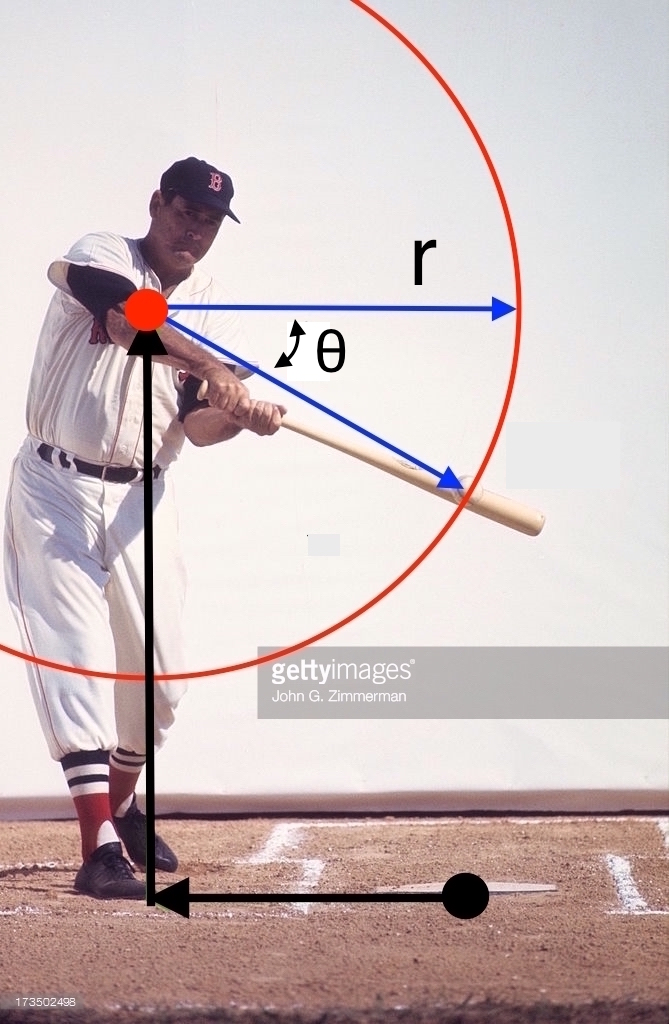
\includegraphics[scale=.15]{Images/WilliamsPolar.jpg} 
	\caption{The ground level black dot represents the origin (0,0) in the rectangular coordinate system. The translated origin (red dot) coincides with the hitter's approximate center of gravity, and thus the polar origin. The bold arrows show the origin shift. The length of the arrows moving out from his center of gravity to specific grid locations represent $r$, and the angle between the same two arrows represent $\theta$.}
	\end{figure} 
Referring to Figure 3, let $r$ measure the distance from the hitter's center of gravity to the ball at impact, and let $\theta$ be the angle below horizontal of the line segment connecting the center of gravity and the ball at impact. As in golf and tennis, ball location---too far/close to the hitter, or above/below the ideal point of impact--- affects hitting performance. Letting $\pmb{X}_{ij}(\pmb{s}_{ij})$ in (1) be comprised of $r_{ij}$ and $\theta_{ij}$ terms provides an exploratory starting point.

\subsubsection{Generalized Linear Model with Biomechanically Interpretable Covariates} % =========================

Let covariate vector $\pmb{X}_{ij}(\pmb{s}_{ij})$ in (1) be defined as $\pmb{X}_{ij}(\pmb{s}_{ij}) = \{r_{ij}, \theta_{ij}, r_{ij}\theta_{ij}, r_{ij}^{2}, \theta_{ij}^{2}, r_{ij}^{2}\theta_{ij}^{2}\}$. Substituting into (1) yields:
\begin{equation}
\text{logit}(p_{ij}|\pmb{s}_{ij}, r_{ij}, \theta_{ij}) = \beta_{j0} + \beta_{j1}r_{ij} + \beta_{j2} \theta_{ij} + \beta_{j3} r_{ij} \theta_{ij} + \beta_{j4}r_{ij}^{2} + \beta_{j5} \theta_{ij}^{2} + \beta_{j6} r_{ij}^{2} \theta_{ij}^{2}
\end{equation}

Note that given a hitter $j$, and pitch location $\pmb{s}_{ij}$, the elements of $\pmb{X}_{ij}$ are simply a trigonemtric function of $\pmb{s}_{ij}$ and the translated origin. Thus, for convenience, we replace $\text{logit}(p_{ij}|\pmb{s}_{ij}, r_{ij}, \theta_{ij})$ with $\text{logit}(p_{ij}|\pmb{s}_{ij})$ for the remainder of this study.

We choose Johnny Peralta from Chapter 1 to illustrate, and let $j = P$ for convenience. We fit model (2) using Peralta's $n_{P} = 9177$ observed swings, find maximum likelihood estimates of $\pmb{\beta}_{P}$ using an iteratively reweighted least squares algorithm \citep{Myers2012}. 

  \begin{figure}[!ht]
    \centering
    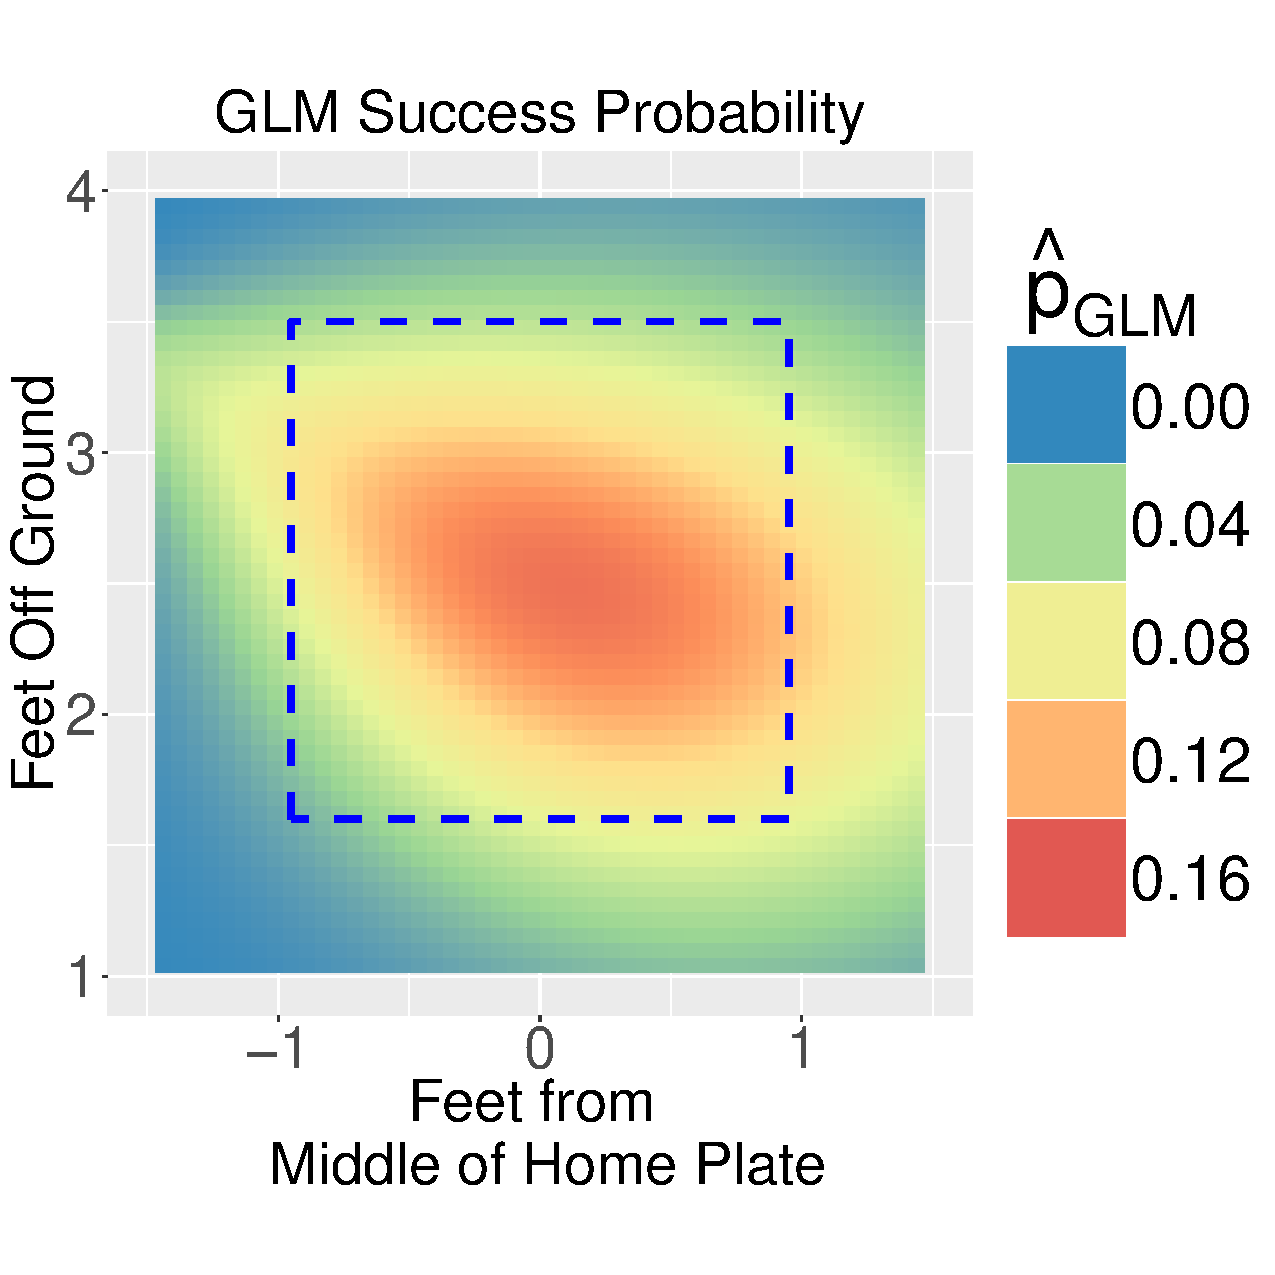
\includegraphics[scale=.25]{Images/Perralta_fit.pdf}
    \qquad
\begin{tabular}[b]{ l | c | c | c | r }
    \hline
    Covariate         & $\beta_{i}$ & MLE   & SE     &      p \\ \hline \hline
    N/A               & $\beta_{0}$ & -4.08 & 0.70 & $ <0.001$ \\ \hline
    r                 & $\beta_{1}$ &  1.19 & 0.51 & $  0.018$ \\ \hline
    $\theta$          & $\beta_{2}$ & -1.93 & 1.90 & $  0.311$ \\ \hline
    $r*\theta$        & $\beta_{3}$ & -1.64 & 0.70 & $  0.064$ \\ \hline
    $r^{2}$           & $\beta_{4}$ & -0.32 & 0.09 & $ <0.001$ \\ \hline
    $\theta^{2}$      & $\beta_{5}$ & -3.92 & 1.10 & $ <0.001$ \\ \hline
    $r^{2}*\theta^{2}$& $\beta_{6}$ & -0.46 & 0.21 & $  0.025$ \\ \hline
    \hline
\end{tabular}
    \captionlistentry[table]{A table beside a figure}
    \captionsetup{labelformat=andtable}
    \caption{A table beside a figure}
  \end{figure}




\subsubsection{Hosmer-Lemeshow Goodness of Fit Test} % ================

Generalized Linear Models \citep{Myers2012}

  \begin{itemize} % ===============
  \item (pg 147) Hosmer-Lemeshow test = Logistic regression Goodness of Fit test. 
  \item Like Pearson Chi-Sq, but for continuous covariates. 
  \item Order all responses according to fitted $\hat{p}$, then group into deciles. 
  \item Then basically $\chi^{2} = \Sigma \Sigma \frac{(O - E)^{2}}{E}$
  \item p-value = 0.1513
  \end{itemize}
  
\subsection{Heat Map Confidence Intervals}

A heat map presents, essentially, a two dimensional surface ``painted'' with point estimates. That is, each (x,y) point on the surface maps a point estimate of a parameter to a color. This effectively communicates the behavior of the parameter, or at least the point estimates, across the spatial domain. However, the usefulness of a point estimate depends on confidence interval accompaniment; and therein lies the challenge: how to present heat map confidence intervals (CIs)? This problem exists across disparate academic areas of research---any area where heat maps are used! ``...question asked in other areas.'' For example, Dr. Sarah Emerson reports that collaborative genomics research with Dr. Yanming Di lacked a satisfactory heat map confidence interval option \citep{Emerson}, (cite paper). Next we present the current heat map CI best practices, and examine why they can and should be improved.

\subsubsection{Current Best Practices}

The currect best practice simply presents the CI lower bound heat map and upper bound heat map, and sometimes maps for additional percentiles. For example, \cite{Cross2015} provides the following collection of heat maps to communicate prediction confidence.

  \begin{figure}[H]
	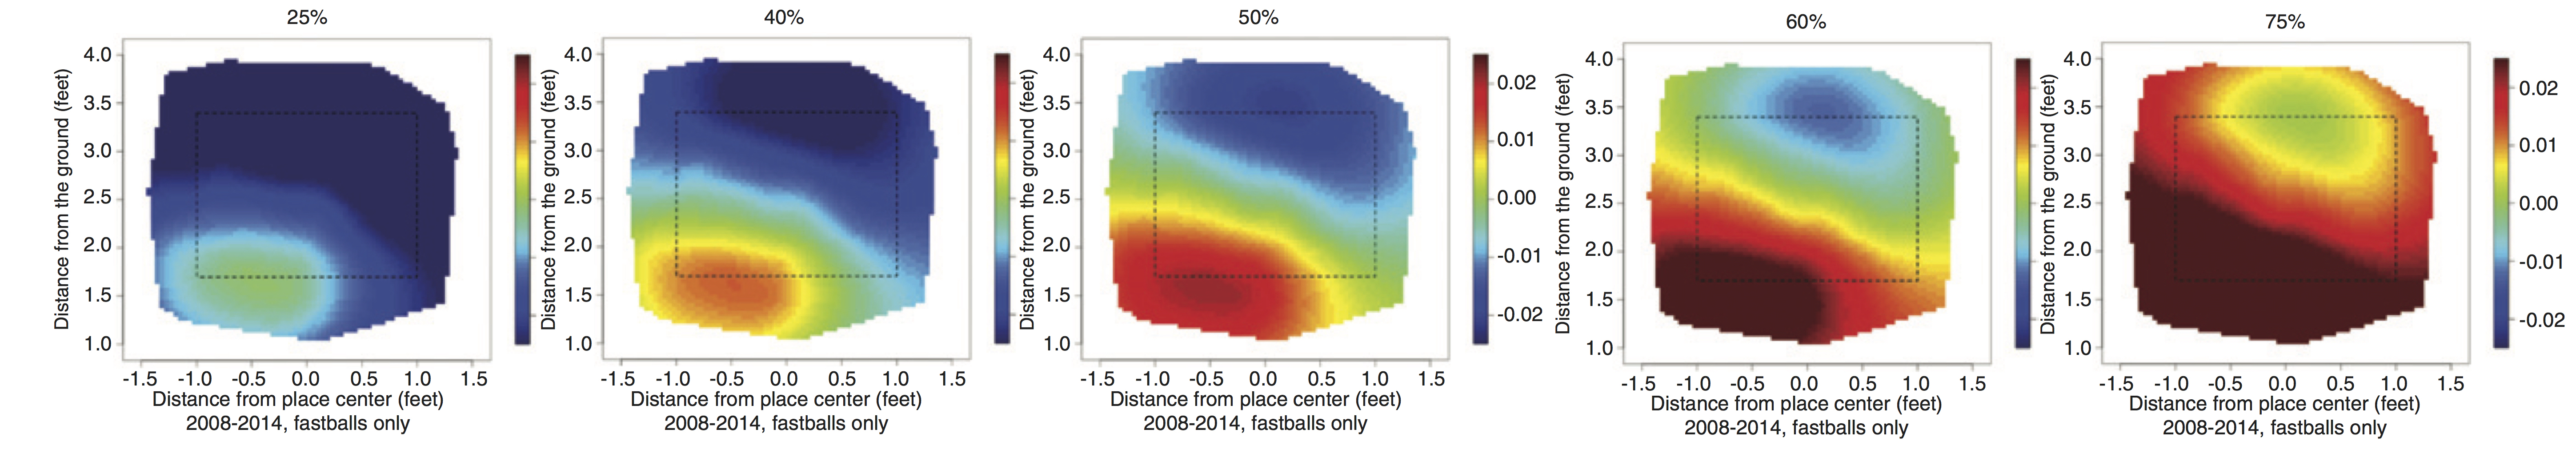
\includegraphics[scale=.085]{Images/CrossHMCI.jpg} 
	\caption{In line with best practices, \cite{Cross2015} present four percentiles to convey confidence interval information for the point estimate heat map in the middle. We submit this method resists easy comprehension and intuition.}
	\end{figure} 
	
This heat map collection, in line with best practices, challenges the viewer on two levels: understanding and intuition. First, one must understand the information begin presented. The two-dimensional, hypothetical point estimate 2, and CI (0,4) makes plain its information content and structure.

  \begin{figure}[H]
  \centering
	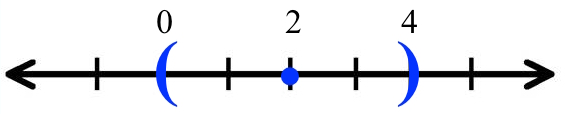
\includegraphics[scale=.6]{Images/NumberLine.jpg} 
	\caption{Our brain readily understands and interprets the content of a confidence interval on the number line. However, the same is not true for the color spectrum.}
	\end{figure}
A point estimate of 2 and CI of (0,4) translates intuitively after so many years using the number line. So, while I quickly, intuitively, and easily understand the content of the number line, this is not necessarily true for the color spectrum. Heat map CIs are less clear because the point estimate and bounds represent parameter values with color; a point estimate of ``green'' with a CI of (purple, red) confounds.

  \begin{figure}[H]
  \centering
	
\includegraphics[scale=.75]{Images/Lower.jpeg} 
	
\includegraphics[scale=.75]{Images/SpectrumPE.jpg} 
	
\includegraphics[scale=.75]{Images/Upper.jpeg} 

	\caption{This representation of a confidence interval on the color spectrum demonstrates the interpretive challenge. What stream of colors exist between each bound and the point estimate?}
	\end{figure}
	
However, the task becomes easier with the segments of the spectrum {\it between} the bounds and point estimate visible, as in Figure XX.
  \begin{figure}[H]
  \centering
	
\includegraphics[scale=.65]{Images/SpectrumCI.jpg} 
	\caption{This representation of a confidence interval on the color spectrum hints at the interpretive solution. Interpretation simplifies with the portions of the color spectrum between each bound and the point estimate visible. The question then---how do we achieve this for a heat map {\it surface}?}
	\end{figure}
This simplifies interpretation immensely. However, the problem remains; how do we acheive this for a heat map surface? A modelled continuous surface essentially maps a limitless number of point estimates to a color, making a visible color spectrum confidence interval for each point estimate infeasible. Nonetheless, we propose a dynamic solution using Shiny, by RStudio \citep{Shiny}, \citep{RStudio}.

\subsubsection{Shiny Innovation}

The inimitable RStudio created the Shiny framework to facilitate interactive web application development. Deployed directly out of the RStudio integrated development environment (IDE) \citep{IDE}, Shiny applications provide statisticians, all scientists in fact, with a powerful new tool for presenting analytical results. We harness a sliver of Shiny's capability to provide a solution to the the heat map CI problem articulated in the previous section.

Recall the GLM fit heat map for Jhony Peralta. Figure 7 shows the lower and upper 95\% pointwise CI heat maps.

  \begin{figure}[H]
	\centering
	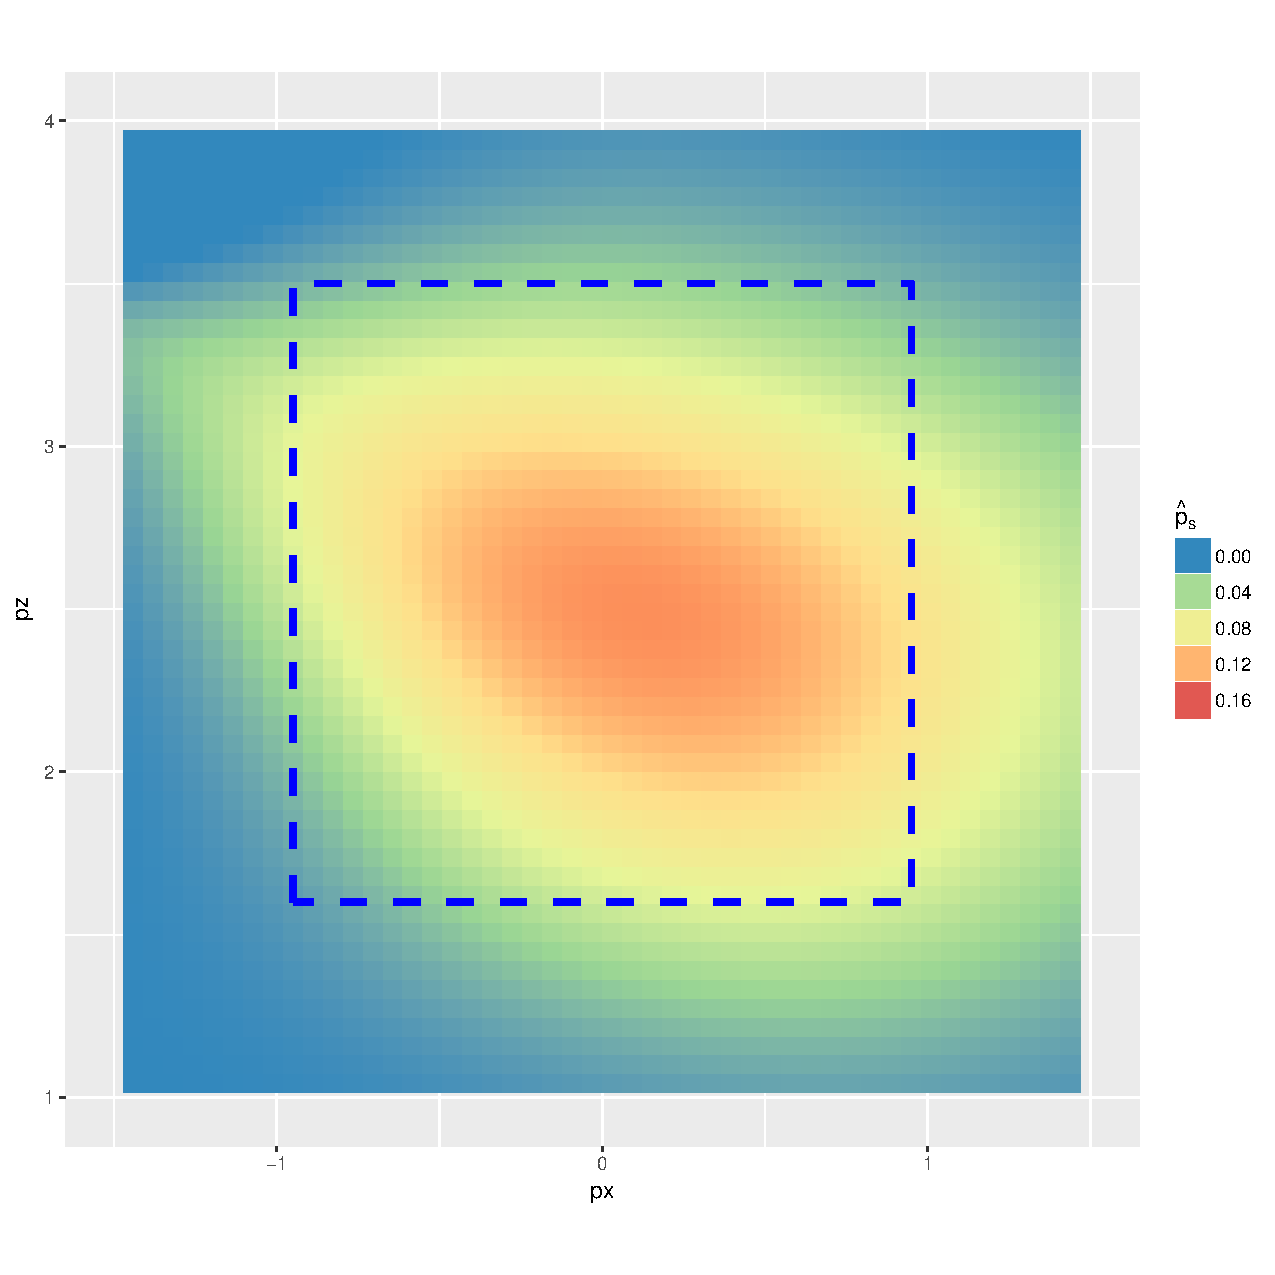
\includegraphics[scale=.25]{Images/Lower.pdf}
	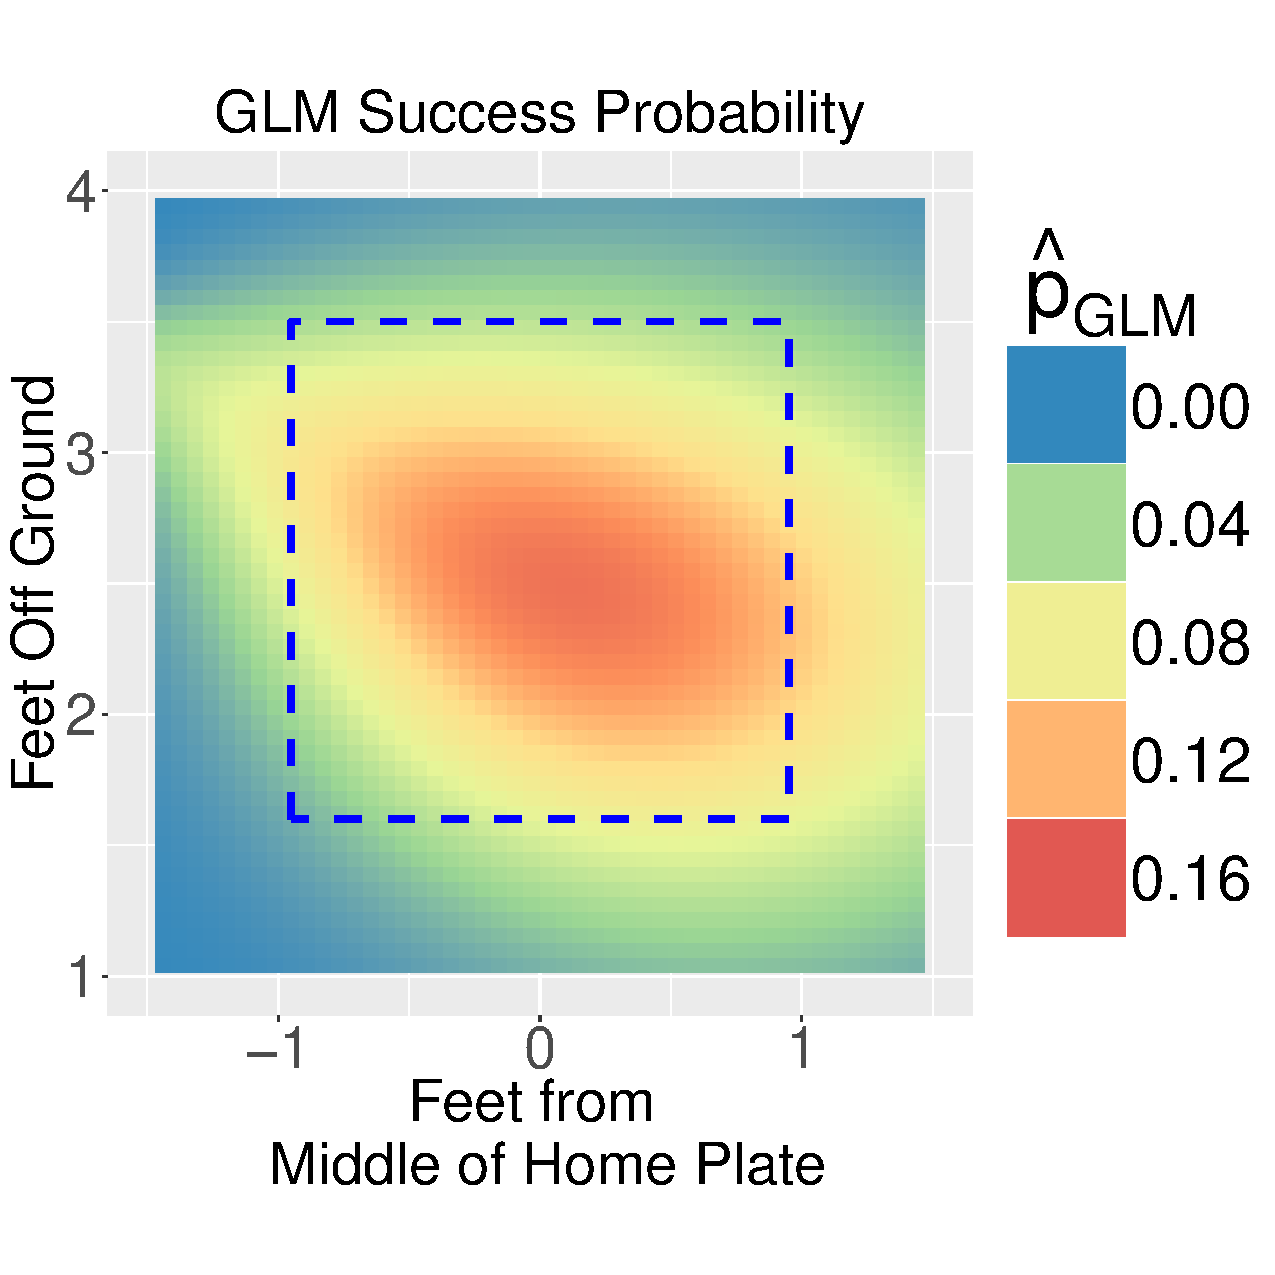
\includegraphics[scale=.25]{Images/Perralta_fit.pdf}
	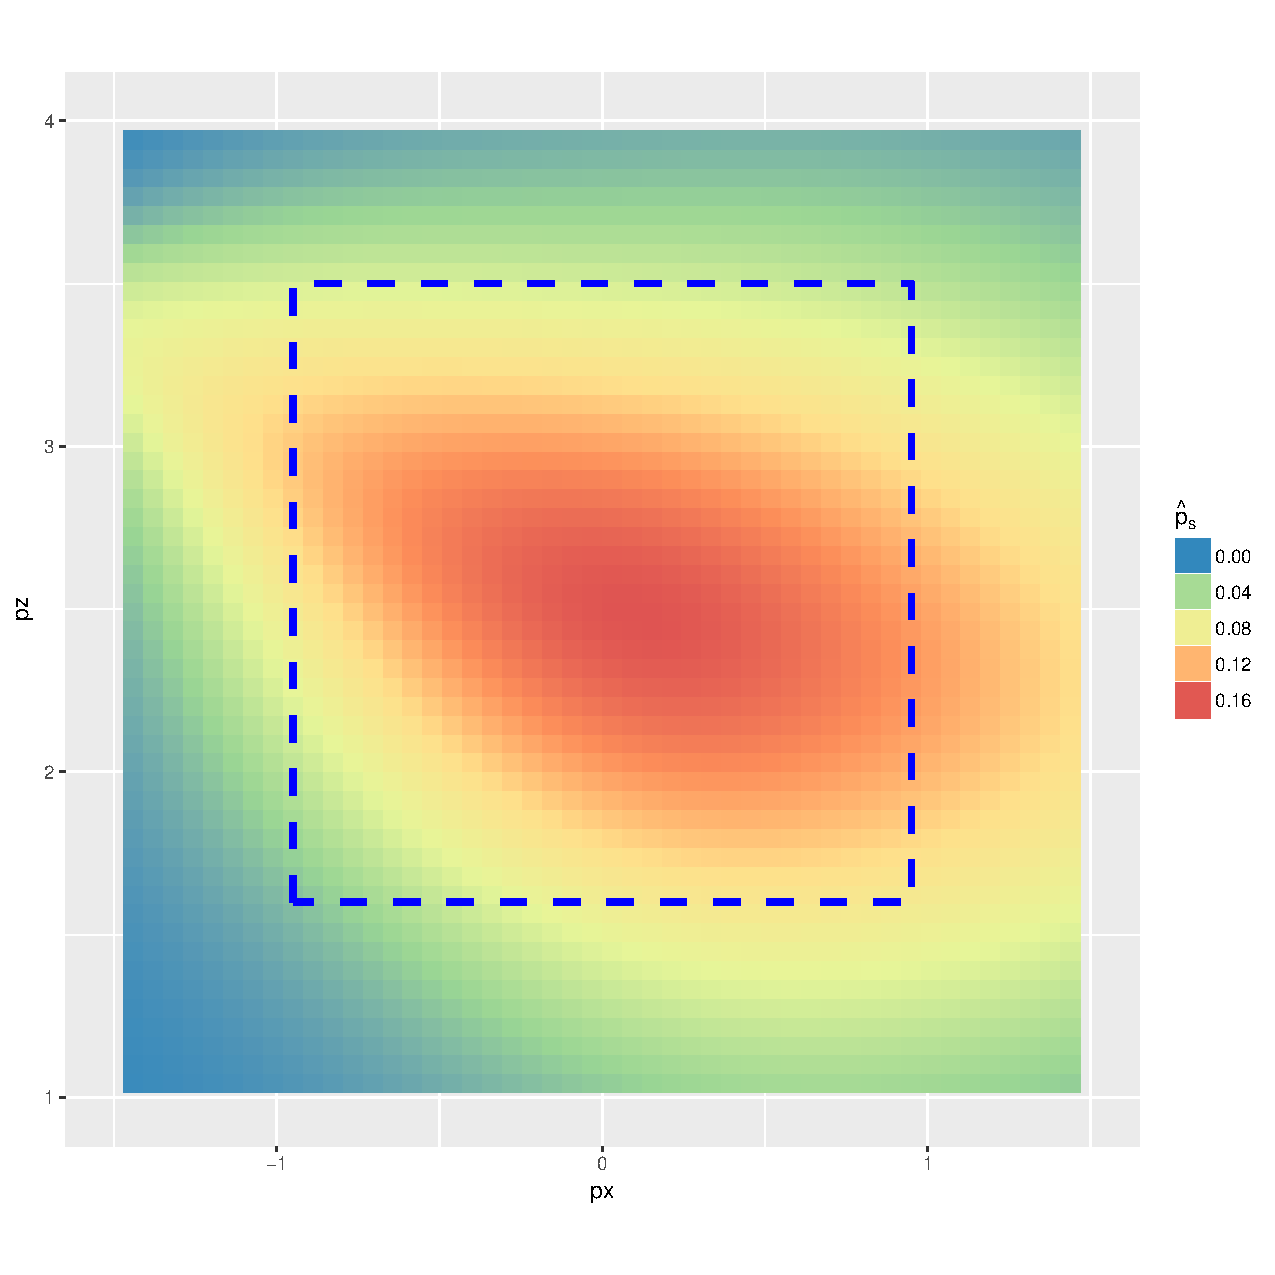
\includegraphics[scale=.25]{Images/Upper.pdf}
	\caption{Current best practices for a heat map confidence interval (CI). The generalized linear model fit for Jhony Peralta in the center, the pointwise CI lower bound on the left, and the pointwise CI upper bound on the right. Our interactive, dynamic heat map CIs will make improve interpretability.} 
	\end{figure}
  
\subsection{Appendix: ShinyHMCI, An R Package}

\bibliography{Baseball}

\end{document}
